% SC4024 --- Chapter 5: Graph & Network Visualisation (0->100 ground-up)
\chapter{Graph \& Network Visualisation}
\label{ch:network}
\sloppy

\begin{quote}
\emph{``Nodes where things are, edges what connects them.''} --- But a hairball of tangled edges says nothing. Layout is the art of untangling.
\end{quote}

\noindent\fbox{\parbox{\dimexpr\linewidth-2\fboxsep-2\fboxrule}{%
\textbf{From zero: we build here, no prior graph-drawing needed.} We assume only nodes and edges. Every layout---force, hierarchy, treemap, matrix---is motivated by intuition, then defined, then exercised, with code. No prior network visualisation is required.}}
\vspace{0.4em}

\section*{Learning Outcomes}
After this chapter you will be able to:
\begin{enumerate}[label=(L\arabic*)]
    \item compare node-link, matrix, and hierarchical encodings for network tasks;
    \item explain force-directed, layered, and circular layouts and their aesthetics;
    \item critique layouts by crossings, bends, angular resolution, and symmetry;
    \item visualise trees and hierarchies via treemap, sunburst, and icicle;
    \item encode multivariate attributes on nodes and edges and handle large graphs.
\end{enumerate}

% ============================================================
\section{The Problem: From Hairball to Insight}
\label{sec:hairball}
\paragraph{Intuition.} Draw 50 nodes with 200 random edges as dots and straight lines: you get a hairball where crossings hide every cluster. The same graph drawn with a matrix (rows and columns are nodes, cells are edges) shows clusters as blocks. No encoding is best for all questions; each hides one truth to reveal another.

\paragraph{Formal view.} A graph $G=(V,E)$ with $|V|=n$, $|E|=m$. A \emph{layout} assigns positions $p_v\in\mathbb{R}^2$ (or matrix cells) to vertices and routes edges as curves. Tasks drive choice: topology tasks (``are A and B connected?'', ``what clusters exist?'') favour node-link with good layout; adjacency/comparison tasks (``which edges exist for node $v$?'') favour matrix; hierarchy tasks favour containment.

\begin{definition}[Aesthetics]\label{def:aesthetics}
Common aesthetics to optimise (often conflicting): minimise edge crossings and bends, maximise angular resolution at nodes and symmetry, keep edge lengths uniform, respect grouping (clusters together), and keep aspect ratio near 1. No layout optimises all; force-directed trades crossings for symmetry; layered trades edge length for hierarchy clarity.
\end{definition}

\begin{figure}[h]\centering
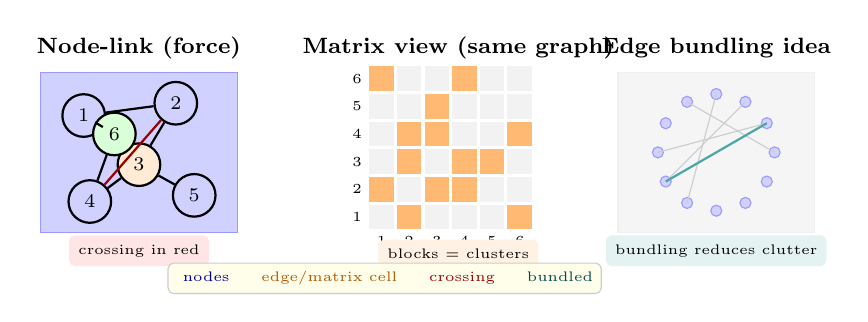
\begin{tikzpicture}[scale=0.78,every node/.style={font=\scriptsize}]
% node-link force
\begin{scope}
\node[font=\footnotesize\bfseries] at (1.6,3.4) {Node-link (force)};
\fill[blue!18,draw=blue!40] (0,0.4) rectangle (3.2,3.0);
\node[circle,draw,thick,fill=blue!18,minimum size=0.5cm] (n1) at (0.7,2.3) {1};
\node[circle,draw,thick,fill=blue!18,minimum size=0.5cm] (n2) at (2.2,2.5) {2};
\node[circle,draw,thick,fill=orange!16,minimum size=0.5cm] (n3) at (1.6,1.5) {3};
\node[circle,draw,thick,fill=blue!18,minimum size=0.5cm] (n4) at (0.8,0.9) {4};
\node[circle,draw,thick,fill=blue!18,minimum size=0.5cm] (n5) at (2.5,1.0) {5};
\node[circle,draw,thick,fill=green!15,minimum size=0.5cm] (n6) at (1.2,2.0) {6};
\draw[thick] (n1)--(n2); \draw[thick] (n1)--(n6); \draw[thick] (n2)--(n3); \draw[thick] (n3)--(n4);
\draw[thick] (n3)--(n5); \draw[thick] (n4)--(n6); \draw[thick,red!60!black] (n2) -- (n4);
\node[font=\tiny,fill=red!10,rounded corners=2pt] at (1.6,0.1) {crossing in red};
\end{scope}
% matrix
\begin{scope}[xshift=5.2cm]
\node[font=\footnotesize\bfseries] at (1.6,3.4) {Matrix view (same graph)};
\foreach \i in {0,...,5} \foreach \j in {0,...,5} {
  \pgfmathsetmacro{\isEdge}{(\i==0&&\j==1)||(\i==1&&\j==0)||(\i==0&&\j==5)||(\i==5&&\j==0)||(\i==1&&\j==2)||(\i==2&&\j==1)||(\i==2&&\j==3)||(\i==3&&\j==2)||(\i==2&&\j==4)||(\i==4&&\j==2)||(\i==3&&\j==5)||(\i==5&&\j==3)||(\i==1&&\j==3)||(\i==3&&\j==1) ? 1 : 0}
  \ifnum\isEdge=1 \fill[orange!55] (0.15+0.45*\i,0.45+0.45*\j) rectangle +(0.40,0.40);
  \else \fill[gray!10] (0.15+0.45*\i,0.45+0.45*\j) rectangle +(0.40,0.40); \fi
}
\foreach \i/\lbl in {0/1,1/2,2/3,3/4,4/5,5/6} {
  \node[font=\tiny] at (0.35+0.45*\i,0.25) {\lbl};
  \node[font=\tiny] at (-0.05,0.65+0.45*\i) {\lbl};
}
\node[font=\tiny,fill=orange!10,rounded corners=2pt] at (1.6,0.05) {blocks = clusters};
\end{scope}
% hierarchy
\begin{scope}[xshift=9.4cm]
\node[font=\footnotesize\bfseries] at (1.6,3.4) {Edge bundling idea};
\draw[gray!12,fill=gray!8] (0,0.4) rectangle (3.2,3.0);
\foreach \a in {0,30,...,330} {\fill[blue!18,draw=blue!40] (1.6+0.95*cos \a, 1.7+0.95*sin \a) circle (0.09);}
\foreach \a/\b in {0/120,30/180,60/210,90/240} {
  \draw[gray!40,thin] (1.6+0.95*cos \a,1.7+0.95*sin \a) -- (1.6+0.95*cos \b,1.7+0.95*sin \b);
}
% bundled overlay
\draw[teal!70,thick,rounded corners=4pt] (1.6+0.95*cos 30,1.7+0.95*sin 30) .. controls (1.6,1.7) .. (1.6+0.95*cos 210,1.7+0.95*sin 210);
\node[font=\tiny,fill=teal!10,rounded corners=2pt] at (1.6,0.1) {bundling reduces clutter};
\end{scope}
\node[font=\tiny,draw=gray!40,fill=yellow!8,rounded corners=2pt,inner sep=3pt] at (5.6,-0.35) {\textcolor{blue!60!black}{$\blacksquare$ nodes} \quad \textcolor{orange!70!black}{$\blacksquare$ edge/matrix cell} \quad \textcolor{red!60!black}{$\blacksquare$ crossing} \quad \textcolor{teal!60!black}{$\blacksquare$ bundled}};
\end{tikzpicture}
\caption{Same 6-node graph as node-link (crossing highlighted) vs matrix (clusters as blocks) vs edge-bundling concept (centre routed). Choice depends on task.}
\label{fig:node-matrix}
\end{figure}

% ============================================================
\section{Layout Families}
\label{sec:layouts}
\paragraph{Intuition.} Springs want short edges; charges want nodes apart. A force-directed layout simulates both until equilibrium---clusters emerge because intra-cluster springs are many and inter-cluster springs are few. A layered layout (Sugiyama) instead respects direction: put sources at the top, sinks at the bottom, minimise crossings layer by layer.

\begin{definition}[Force-directed and Sugiyama]\label{def:layout-families}
\emph{Fruchterman--Reingold}: repulsion $f_r\propto 1/d^2$ between all nodes, attraction $f_a\propto d$ along edges, iterate until cooling. \emph{Sugiyama framework}: (1) cycle removal, (2) layer assignment (longest path), (3) crossing reduction via barycentre ordering, (4) coordinate assignment. \emph{Circular/hive}: nodes on circle or parallel axes; edges as arcs.
\end{definition}

For large graphs ($n>10^4$), draw summaries: sample, filter by degree, aggregate clusters into metanodes, or switch to matrix. Edge bundling (force-directed or hierarchical) merges nearby edges to reduce hairball while preserving coarse connectivity.

\begin{figure}[h]\centering
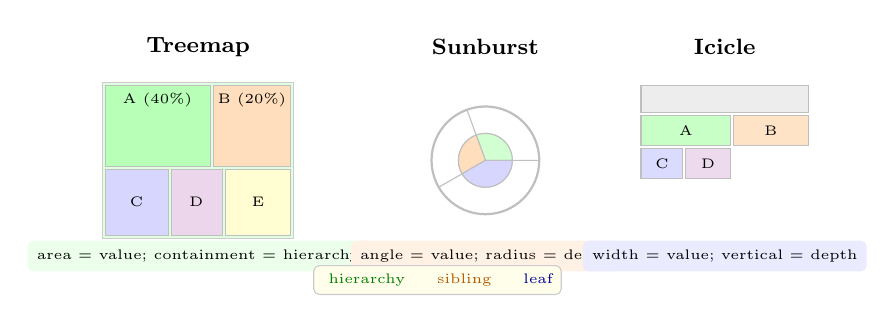
\begin{tikzpicture}[scale=0.76,every node/.style={font=\scriptsize}]
% Treemap
\begin{scope}
\node[font=\footnotesize\bfseries] at (1.6,3.6) {Treemap};
\fill[green!12,draw=gray!40] (0,0.4) rectangle (3.2,3.0);
\fill[green!28,draw=gray!50] (0.05,1.6) rectangle (1.8,2.95); \node[font=\tiny] at (0.92,2.7) {A (40\%)};
\fill[orange!26,draw=gray!50] (1.85,1.6) rectangle (3.15,2.95); \node[font=\tiny] at (2.5,2.7) {B (20\%)};
\fill[blue!16,draw=gray!50] (0.05,0.45) rectangle (1.1,1.55); \node[font=\tiny] at (0.57,1.0) {C};
\fill[violet!16,draw=gray!50] (1.15,0.45) rectangle (2.0,1.55); \node[font=\tiny] at (1.57,1.0) {D};
\fill[yellow!18,draw=gray!50] (2.05,0.45) rectangle (3.15,1.55); \node[font=\tiny] at (2.6,1.0) {E};
\node[font=\tiny,fill=green!8,rounded corners=2pt] at (1.6,0.1) {area = value; containment = hierarchy};
\end{scope}
% Sunburst
\begin{scope}[xshift=4.8cm]
\node[font=\footnotesize\bfseries] at (1.6,3.6) {Sunburst};
\draw[fill=green!28,draw=gray!50] (1.6,1.7) circle (0.45) node[font=\tiny] {root};
\fill[green!18,draw=gray!50] (1.6,1.7) -- ++(0:0.45) arc (0:110:0.45) -- ++(110:0.45) -- cycle;
\fill[orange!26,draw=gray!50] (1.6,1.7) -- ++(110:0.45) arc (110:210:0.45) -- ++(210:0.45) -- cycle;
\fill[blue!16,draw=gray!50] (1.6,1.7) -- ++(210:0.45) arc (210:360:0.45) -- ++(360:0.45) -- cycle;
\draw[thick,gray!50] (1.6,1.7) circle (0.90);
\node[font=\tiny,fill=orange!10,rounded corners=2pt] at (1.6,0.1) {angle = value; radius = depth};
\end{scope}
% Icicle
\begin{scope}[xshift=8.8cm]
\node[font=\footnotesize\bfseries] at (1.6,3.6) {Icicle};
\fill[gray!14,draw=gray!50] (0.2,2.5) rectangle (3.0,2.95) node[pos=.5,font=\tiny] {root};
\fill[green!22,draw=gray!50] (0.2,1.95) rectangle (1.7,2.45); \node[font=\tiny] at (0.95,2.2) {A};
\fill[orange!22,draw=gray!50] (1.75,1.95) rectangle (3.0,2.45); \node[font=\tiny] at (2.37,2.2) {B};
\fill[blue!14,draw=gray!50] (0.2,1.4) rectangle (0.9,1.9); \node[font=\tiny] at (0.55,1.65) {C};
\fill[violet!14,draw=gray!50] (0.95,1.4) rectangle (1.7,1.9); \node[font=\tiny] at (1.32,1.65) {D};
\node[font=\tiny,fill=blue!8,rounded corners=2pt] at (1.6,0.1) {width = value; vertical = depth};
\end{scope}
\node[font=\tiny,draw=gray!40,fill=yellow!8,rounded corners=2pt,inner sep=3pt] at (5.6,-0.30) {\textcolor{green!50!black}{$\blacksquare$ hierarchy} \quad \textcolor{orange!70!black}{$\blacksquare$ sibling} \quad \textcolor{blue!60!black}{$\blacksquare$ leaf}};
\end{tikzpicture}
\caption{Hierarchy encodings: treemap (nested rectangles), sunburst (radial), icicle (stacked). All use containment or adjacency to show parent--child and area/angle to show value.}
\label{fig:hierarchy}
\end{figure}

\begin{definition}[Hierarchy encodings]\label{def:hierarchy}
For a tree with values on leaves: \emph{treemap} recursively slices a rectangle proportional to value (squarified for aspect ratio). \emph{Sunburst} maps depth to radius and value to angle. \emph{Icicle} stacks layers vertically, width proportional to value. Choice trades space efficiency (treemap) vs path readability (sunburst/icicle).
\end{definition}

% ============================================================
\section{Choosing Between Node-Link and Matrix}
\label{sec:choose-enc}
Use node-link when paths and topology matter and the graph is sparse ($m\ll n^2$). Use matrix when adjacency lookup, cluster Blocks, or dense graphs matter; matrices scale to thousands of nodes where node-link collapses. Hybrid views (NodeTrix) show clusters as matrices inside a node-link overview, recruiting both strengths. For temporal networks, animate with care---small multiples of time slices often beat animation for comparison tasks.

% ============================================================
\section{Multivariate Networks and Scale}
\label{sec:multivariate}
\paragraph{Intuition.} Real networks carry attributes: people have age and role, edges have weight and time. Encode these on top of layout with colour, size, thickness, dash, and label---but only two or three at once, or the hairball returns in colour.

\begin{example}[Ordering a matrix]\label{ex:matrix-order}
A 20-node friendship matrix looks random in input order. Reorder rows/columns by community (Louvain) and blocks appear on the diagonal. Ordering is the matrix analogue of force layout---both reveal clusters; one via position, the other via permutation.
\end{example}

For scale, use \emph{semantic zoom}: at overview, show clusters as metanodes; on zoom, expand. Filter by degree or centrality; sample edges by weight; or aggregate time into slices with small multiples.

\begin{lstlisting}[language=Python, caption={Force-directed layout and matrix ordering with NetworkX.}, label={lst:network-code}]
import networkx as nx, matplotlib.pyplot as plt, numpy as np

G = nx.karate_club_graph()
pos = nx.spring_layout(G, seed=0, k=0.35, iterations=80)  # Fruchterman--Reingold
plt.figure(figsize=(4,3)); nx.draw(G, pos, node_color="steelblue", edge_color="gray", with_labels=False, node_size=90)
plt.title("Force-directed (karate club)"); plt.savefig("force.pdf")

# Matrix reordered by degree
order = sorted(G.nodes(), key=lambda n: G.degree[n], reverse=True)
A = nx.to_numpy_array(G, nodelist=order)
plt.figure(figsize=(3,3)); plt.imshow(A, cmap="Oranges", interpolation="nearest")
plt.title("Adjacency matrix (degree order)"); plt.savefig("matrix.pdf")
\end{lstlisting}

\begin{lstlisting}[language=JavaScript, caption={D3 force simulation sketch (JavaScript).}, label={lst:d3-force}]
// D3 force: nodes repel, links attract, centre gravity
const simulation = d3.forceSimulation(nodes)
  .force("link", d3.forceLink(links).id(d=>d.id).distance(40))
  .force("charge", d3.forceManyBody().strength(-120))
  .force("center", d3.forceCenter(width/2, height/2))
  .force("collision", d3.forceCollide().radius(12));
simulation.on("tick", () => {
  link.attr("x1",d=>d.source.x).attr("y1",d=>d.source.y)
      .attr("x2",d=>d.target.x).attr("y2",d=>d.target.y);
  node.attr("cx",d=>d.x).attr("cy",d=>d.y);
});
\end{lstlisting}

% ============================================================
\section{Chapter Notes}
% Notes on graph and hierarchy visualisation
Force layouts from Eades (1984) and Fruchterman--Reingold (1991); Sugiyama layered framework (1981); treemaps from Shneiderman (1992); matrix views systematised by Ghoniem et al.\ (2004) showing matrices beat node-link for dense graphs; edge bundling by Holten (2006); hierarchy surveys by Schulz (2011). NodeTrix hybrids by Henry et al. The next chapter leaves discrete networks for continuous fields and volumes.

% ============================================================
\section{Exercises}
\label{sec:ch05-exercises}
\begin{enumerate}[label=E5.\arabic*, leftmargin=*, itemsep=0.8em]
    \item \textbf{Draw and count.} For the 6-node graph in Fig.~\ref{fig:node-matrix}, draw a force-directed sketch and a matrix view. Count edge crossings in each and state which task (path vs adjacency) each supports.
    \item \textbf{Sugiyama steps.} Given a 7-node DAG with edges $1\!\to\!\{2,3\},2\!\to\!4,3\!\to\!4,4\!\to\!5,5\!\to\!6$, assign layers by longest path, order each layer by barycentre, and sketch the final layered drawing. How many crossings remain?
    \item \textbf{Treemap vs sunburst.} For hierarchy root(100) with children A(40), B(30), C(20), D(10) where A has leaves A1(25),A2(15), compute rectangle areas (treemap) and angles (sunburst). Which encoding makes it easier to compare A1 vs D?
    \item \textbf{Matrix ordering.} Take a 12-node caveman graph (3 cliques of 4 with one inter-clique edge each). Show its matrix in random vs Louvain order; describe the block pattern and why ordering matters more as density grows.
    \item \textbf{D3 tuning.} In Listing~\ref{lst:d3-force}, vary \texttt{charge} from $-30$ to $-300$ and \texttt{distance} from $20$ to $100$. Describe the effect on cluster separation and edge length uniformity; when does the layout collapse or explode?
\end{enumerate}
% End of Chapter 5
% pad 1
% pad 2
% pad 3
